% The 2026 Midterms: how it works, the ads, and the results
% Compile with: latexmk -pdf midterms_2026.tex
\documentclass[aspectratio=169,11pt]{beamer}

\usepackage[T1]{fontenc}
\usepackage{lmodern}
\usepackage{booktabs}
\usepackage{array}
\usepackage{tikz}
\usetikzlibrary{shapes.geometric,positioning,calc,arrows.meta,patterns}
\usepackage{pgfplots}
\pgfplotsset{compat=1.18}
\usepackage[most]{tcolorbox}
\graphicspath{{images/}}

% ---------- Colors ----------
\definecolor{navy}{HTML}{1C2541}
\definecolor{oldred}{HTML}{B22234}
\definecolor{oldblue}{HTML}{3C3B6E}
\definecolor{ink}{HTML}{2B2B2B}
\definecolor{muted}{HTML}{8A8F98}
\definecolor{paper}{HTML}{FFFFFF}
\definecolor{dem}{HTML}{2E5FA3}
\definecolor{rep}{HTML}{C0392B}

% ---------- Minimal theme ----------
\setbeamertemplate{navigation symbols}{}
\setbeamercolor{normal text}{fg=ink, bg=paper}
\setbeamercolor{structure}{fg=navy}
\setbeamercolor{frametitle}{fg=navy}
\setbeamercolor{alerted text}{fg=oldred}
\setbeamercolor{footnote}{fg=muted}
\setbeamerfont{frametitle}{size=\Large, series=\bfseries}
\setbeamertemplate{itemize item}{\color{oldred}\textbullet}
\setbeamertemplate{itemize subitem}{\color{muted}--}
\setbeamertemplate{enumerate item}{\color{oldred}\insertenumlabel.}
\setbeamersize{text margin left=1.1cm, text margin right=1.1cm}
\hypersetup{colorlinks=true, urlcolor=dem, linkcolor=navy}

\setbeamertemplate{frametitle}{%
  \vspace*{0.5cm}%
  \usebeamerfont{frametitle}\usebeamercolor[fg]{frametitle}\insertframetitle\par
  \vspace{0.15cm}{\color{navy!15}\rule{\textwidth}{0.4pt}}\par}

\setbeamertemplate{footline}{%
  \hfill{\tiny\color{muted}\insertframenumber}\hspace*{0.6cm}\vspace*{0.35cm}}

% Plain divider at the start of each section
\AtBeginSection{%
  \begin{frame}[plain,noframenumbering]
    \centering
    {\LARGE\bfseries\color{navy}\insertsection}\\[0.6em]
    {\color{oldred}\rule{1.5cm}{0.8pt}}
  \end{frame}}

% "Think" question slides
\newenvironment{thinkframe}{%
  \begin{frame}[plain,noframenumbering,environment=thinkframe]\centering\Large}{\end{frame}}

% ---------- Helpers ----------
% Small grey source line at the bottom of a frame
\newcommand{\source}[1]{%
  \begin{tikzpicture}[remember picture,overlay]
    \node[anchor=south west, font=\tiny, text=muted, text width=0.85\paperwidth, align=left]
      at ($(current page.south west)+(0.6cm,0.25cm)$) {#1};
  \end{tikzpicture}}

% Quote box with a thin red rule on the left
\newtcolorbox{textquote}[1][]{%
  enhanced, frame hidden, boxrule=0pt, sharp corners,
  colback=navy!4, borderline west={2pt}{0pt}{oldred},
  left=10pt, right=8pt, top=6pt, bottom=6pt, fontupper=\itshape, #1}

% Candidate card: photo, name, two lines of bio
\newcommand{\candidate}[3]{%
  \begin{minipage}[t]{\linewidth}\centering
    \includegraphics[height=3.5cm]{#1}\\[0.5em]
    {\large\bfseries\color{navy}#2}\\[0.4em]
    \begin{minipage}{0.9\linewidth}\raggedright\small #3\end{minipage}
  \end{minipage}}

% Big number with a caption
\newcommand{\bignum}[3]{%
  \begin{minipage}[t]{\linewidth}\centering
    {\fontsize{34}{38}\selectfont\bfseries\color{#1}#2}\\[0.3em]
    {\small #3}
  \end{minipage}}

% Ad slide: \adframe{number}{race}{thumbnail}{YouTube id}{offline file}{reveal bullets}
\newcommand{\adframe}[6]{%
  \begin{frame}{Ad #1: #2}
    \begin{columns}[T]
      \begin{column}{0.56\textwidth}
        \centering
        \href{https://youtu.be/#4}{%
          \begin{tikzpicture}
            \node[inner sep=0pt] (t) {\includegraphics[width=\linewidth,height=4.4cm,keepaspectratio]{#3}};
            \fill[black, opacity=0.55] (t.center) circle (0.62cm);
            \fill[white] ($(t.center)+(-0.18,0.3)$) -- ($(t.center)+(-0.18,-0.3)$) -- ($(t.center)+(0.33,0)$) -- cycle;
          \end{tikzpicture}}\\[0.3em]
        {\tiny\color{muted} Click to play: youtu.be/\detokenize{#4} \textbullet\ Offline: ads/#5\par}
      \end{column}
      \begin{column}{0.4\textwidth}
        \begin{minipage}[t][5cm][t]{\linewidth}
          \only<1>{
            {\bfseries\color{oldred}Your vote}
            \begin{enumerate}\setlength{\itemsep}{0.9em}
              \item Positive or attack?
              \item Fear, anger, laughter or trust?
              \item Will it work? \textbf{Write it down!}
            \end{enumerate}}
          \only<2>{
            {\bfseries\color{navy}The answer}
            \begin{itemize}\setlength{\itemsep}{0.6em}\small
              #6
            \end{itemize}}
        \end{minipage}
      \end{column}
    \end{columns}
  \end{frame}}

% Big guess / reveal slide: \guess{question}{answer}{caption}
\newcommand{\guess}[3]{%
  \begin{frame}[plain]
    \vfill
    \begin{center}
      {\small\bfseries\color{oldred}Guess}\\[0.8em]
      {\LARGE\bfseries\color{navy}#1}\\[1.6em]
      \uncover<2->{{\fontsize{40}{44}\selectfont\bfseries\color{oldred}#2}\\[0.6em]
      {\normalsize\color{muted}#3}}
    \end{center}
    \vfill
  \end{frame}}

% Candidate card for the final activity
\newcommand{\card}[3]{%
  \begin{tikzpicture}
    \node[draw=navy!30, line width=0.6pt, rounded corners=4pt, fill=navy!3,
          minimum width=4.1cm, minimum height=2.7cm, text width=3.7cm, align=center] {%
      {\fontsize{20}{22}\selectfont #1}\\[0.3em]
      {\bfseries\color{navy}#2}\\[0.3em]
      {\footnotesize\color{muted}#3}};
  \end{tikzpicture}}

% ---------- Title ----------
\title{The 2026 Midterm Elections}
\author{}
\date{}

\begin{document}

\begin{frame}[plain]
  \begin{columns}[c]
    \begin{column}{0.56\textwidth}
      {\fontsize{30}{34}\selectfont\bfseries\color{navy} The 2026\\Midterms}\\[0.8em]
      {\Large\color{muted} How it works, the ads,\\and who won}\\[0.6em]
      {\color{oldred}\rule{3cm}{1.5pt}}
    \end{column}
    \begin{column}{0.4\textwidth}
      \centering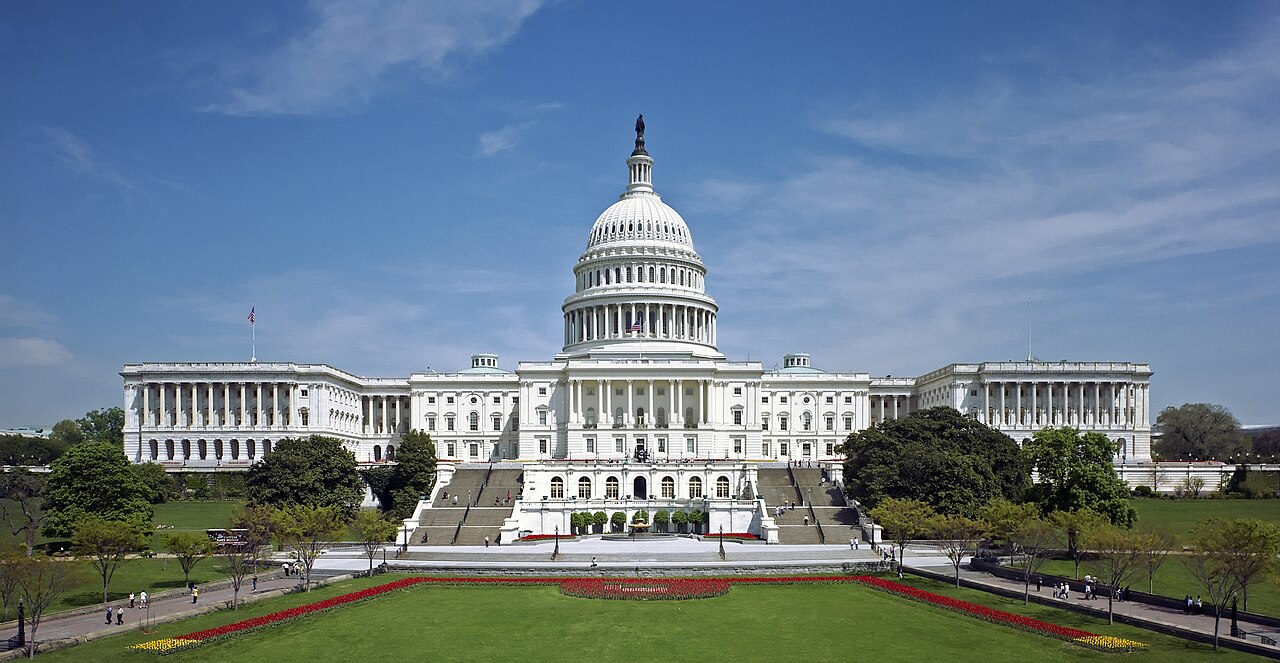
\includegraphics[width=\linewidth]{capitol.jpg}
    \end{column}
  \end{columns}
\end{frame}

% =====================================================================
\section{Warm-up}

\begin{frame}{Maine: who would you vote for?}
  \begin{columns}[T]
    \begin{column}{0.45\textwidth}
      \candidate{jackson.jpg}{Troy Jackson (D)}{%
        \begin{itemize}
          \item Logger from northern Maine
          \item Wants Medicare for All
        \end{itemize}}
    \end{column}
    \begin{column}{0.45\textwidth}
      \candidate{collins.jpg}{Susan Collins (R)}{%
        \begin{itemize}
          \item Senator since 1997
          \item Often votes against her party
        \end{itemize}}
    \end{column}
  \end{columns}
  \vfill
  \begin{center}\alert{\textbf{Hands up!}} We'll see what Maine decided.\end{center}
\end{frame}

% =====================================================================
\section{How It Works}

\begin{frame}{Three branches of government}
  \relax The branches \alert{check and balance} each other. In 2026: \textbf{\color{oldred}Congress} was on the ballot.
  \vfill
  \centering
  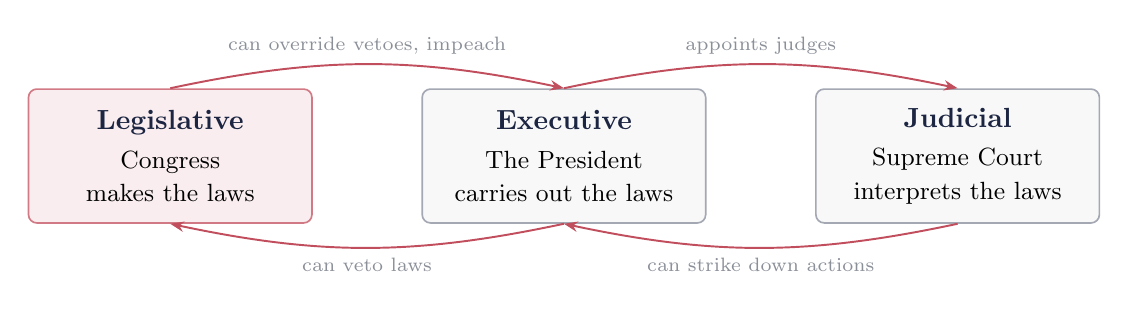
\begin{tikzpicture}[
      box/.style={draw=navy!40, line width=0.6pt, rounded corners=3pt, minimum width=3.6cm,
                  minimum height=1.7cm, align=center, fill=navy!3},
      chk/.style={-{Stealth[length=5pt]}, oldred!80, line width=0.7pt, bend left=12}]
    \node[box, fill=oldred!8, draw=oldred!60] (L) at (0,0) {\textbf{\color{navy}Legislative}\\[0.2em]\small Congress\\\small makes the laws};
    \node[box] (E) at (5,0) {\textbf{\color{navy}Executive}\\[0.2em]\small The President\\\small carries out the laws};
    \node[box] (J) at (10,0) {\textbf{\color{navy}Judicial}\\[0.2em]\small Supreme Court\\\small interprets the laws};
    \draw[chk] (L.north) to node[above, font=\scriptsize, text=muted] {can override vetoes, impeach} (E.north);
    \draw[chk] (E.south) to node[below, font=\scriptsize, text=muted] {can veto laws} (L.south);
    \draw[chk] (E.north) to node[above, font=\scriptsize, text=muted] {appoints judges} (J.north);
    \draw[chk] (J.south) to node[below, font=\scriptsize, text=muted] {can strike down actions} (E.south);
  \end{tikzpicture}
  \vfill
\end{frame}

\begin{frame}{Congress: two chambers}
  \begin{columns}[c]
    \begin{column}{0.55\textwidth}
      \begin{itemize}\setlength{\itemsep}{0.8em}
        \item \textbf{House of Representatives}
          \begin{itemize}
            \item 435 members, 2-year terms
            \item Seats by population
          \end{itemize}
        \item \textbf{Senate}
          \begin{itemize}
            \item 100 members, 6-year terms
            \item 2 per state, any size
          \end{itemize}
      \end{itemize}
    \end{column}
    \begin{column}{0.4\textwidth}
      \centering
      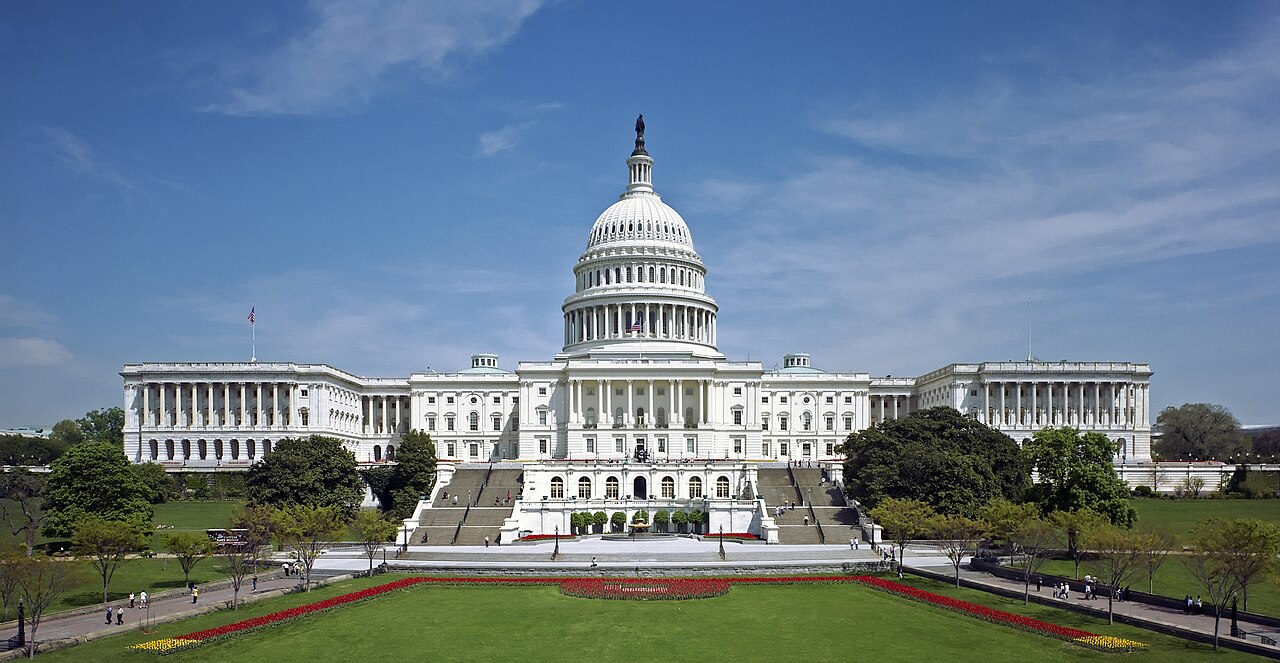
\includegraphics[width=\linewidth]{capitol.jpg}\\[0.2em]
      {\tiny\color{muted} The U.S.\ Capitol, Washington, D.C.\par}
    \end{column}
  \end{columns}
\end{frame}

\begin{frame}{Compare: the USA and Austria}
  \centering
  \renewcommand{\arraystretch}{1.5}
  \begin{tabular}{@{}>{\raggedright\arraybackslash}p{0.27\textwidth}>{\raggedright\arraybackslash}p{0.32\textwidth}>{\raggedright\arraybackslash}p{0.32\textwidth}@{}}
    \toprule
    & \textbf{\color{oldblue}USA} & \textbf{\color{oldred}Austria} \\
    \midrule
    Who runs the government? & The President & The Chancellor \\
    How are they chosen? & Elected separately from Congress & Needs a majority in the \emph{Nationalrat} \\
    Head of state & The President (same person) & The Federal President \\
    National elections & Every \alert{2} years & Every 5 years \\
    \bottomrule
  \end{tabular}
\end{frame}

\begin{frame}{What is a midterm?}
  \begin{itemize}\setlength{\itemsep}{1em}
    \item Halfway through the President's \textbf{four-year} term
    \item All \alert{435} House seats
    \item About \alert{one third} of the Senate
    \item 2026: Tuesday, \textbf{November 3}
    \item The President is \alert{not} on the ballot
  \end{itemize}
\end{frame}

\begin{frame}[plain]
  \vfill
  \begin{center}
    {\small\bfseries\color{oldred}Guess}\\[0.8em]
    {\LARGE\bfseries\color{navy}In the last 20 midterms, how often did\\the President's party \emph{lose} House seats?}
  \end{center}
  \vfill
\end{frame}

\begin{frame}{18 of 20 times}
  \centering
  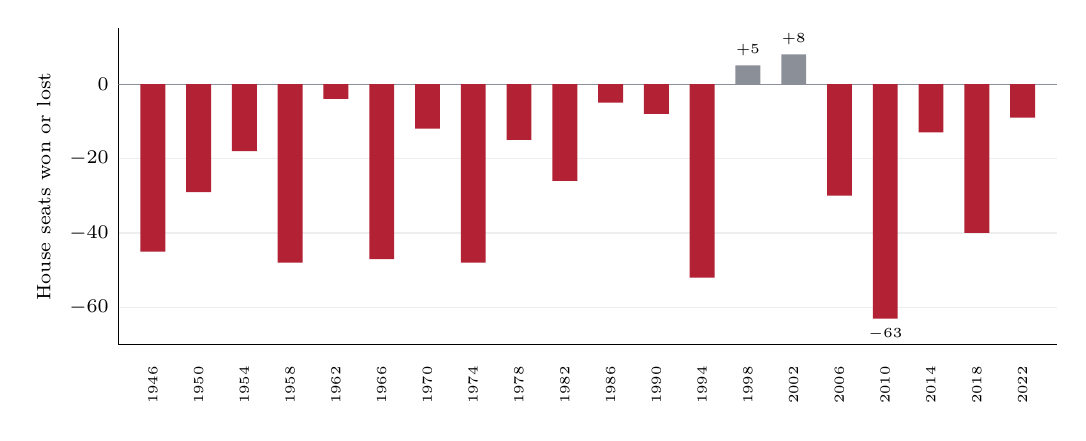
\begin{tikzpicture}
    \begin{axis}[
        ybar, width=13.5cm, height=5.6cm, bar width=9pt,
        ymin=-70, ymax=15, xmin=1943, xmax=2025,
        axis x line*=bottom, axis y line*=left,
        xtick={1946,1950,...,2022}, x tick label style={font=\tiny, rotate=90, anchor=east, /pgf/number format/1000 sep={}},
        ytick={-60,-40,-20,0}, y tick label style={font=\scriptsize},
        ymajorgrids, grid style={navy!8},
        ylabel={\scriptsize House seats won or lost}, tick style={draw=none}]
      \draw[muted] (axis cs:1943,0) -- (axis cs:2025,0);
      \addplot[fill=oldred, draw=none, bar shift=0pt] coordinates {
        (1946,-45) (1950,-29) (1954,-18) (1958,-48) (1962,-4) (1966,-47) (1970,-12)
        (1974,-48) (1978,-15) (1982,-26) (1986,-5) (1990,-8) (1994,-52)
        (2006,-30) (2010,-63) (2014,-13) (2018,-40) (2022,-9)};
      \addplot[fill=muted, draw=none, bar shift=0pt] coordinates {(1998,5) (2002,8)};
      \node[font=\tiny, anchor=north] at (axis cs:2010,-63) {$-$63};
      \node[font=\tiny, anchor=south] at (axis cs:1998,5) {+5};
      \node[font=\tiny, anchor=south] at (axis cs:2002,8) {+8};
    \end{axis}
  \end{tikzpicture}

  \vspace{0.3em}
  \small Voters swing \alert{against the party in power}. Unpopular President? Average loss: \alert{37 seats}.
  \source{Sources: University of Michigan Center for Political Studies; Gallup.}
\end{frame}

% =====================================================================
\section{The Campaign}

\begin{frame}{The starting line}
  \begin{columns}[T]
    \begin{column}{0.28\textwidth}
      \bignum{rep}{53--47}{Senate\\\color{muted}Republican majority}
    \end{column}
    \begin{column}{0.38\textwidth}
      \bignum{rep}{\mbox{218--214}}{House\\\color{muted}Republican majority}
    \end{column}
    \begin{column}{0.28\textwidth}
      \bignum{navy}{38\%}{Trump approval\\\color{muted}on election day}
    \end{column}
  \end{columns}
  \vspace{1.6em}
  \begin{center}
    Democrats needed \alert{4 more} Senate seats.\\[0.3em]
    \uncover<2->{Betting markets on Nov.\ 2: \alert{74\%} chance they'd do it.}
  \end{center}
  \source{Sources: Gallup; NBC/CBS exit polls (approval); Kalshi and Polymarket, Nov.\ 2. House: seats filled before the election.}
\end{frame}

\begin{frame}{The map war}
  \begin{columns}[c]
    \begin{column}{0.55\textwidth}
      \begin{itemize}\setlength{\itemsep}{0.9em}
        \item States draw their own \textbf{House districts}
        \item \alert{Gerrymandering}: lines that favor one party
        \item 2025: Texas redrew for \alert{+5 Republicans}
        \item California answered: \alert{+5 Democrats}
        \item On paper: about +9 Republican
      \end{itemize}
    \end{column}
    \begin{column}{0.4\textwidth}
      \centering
      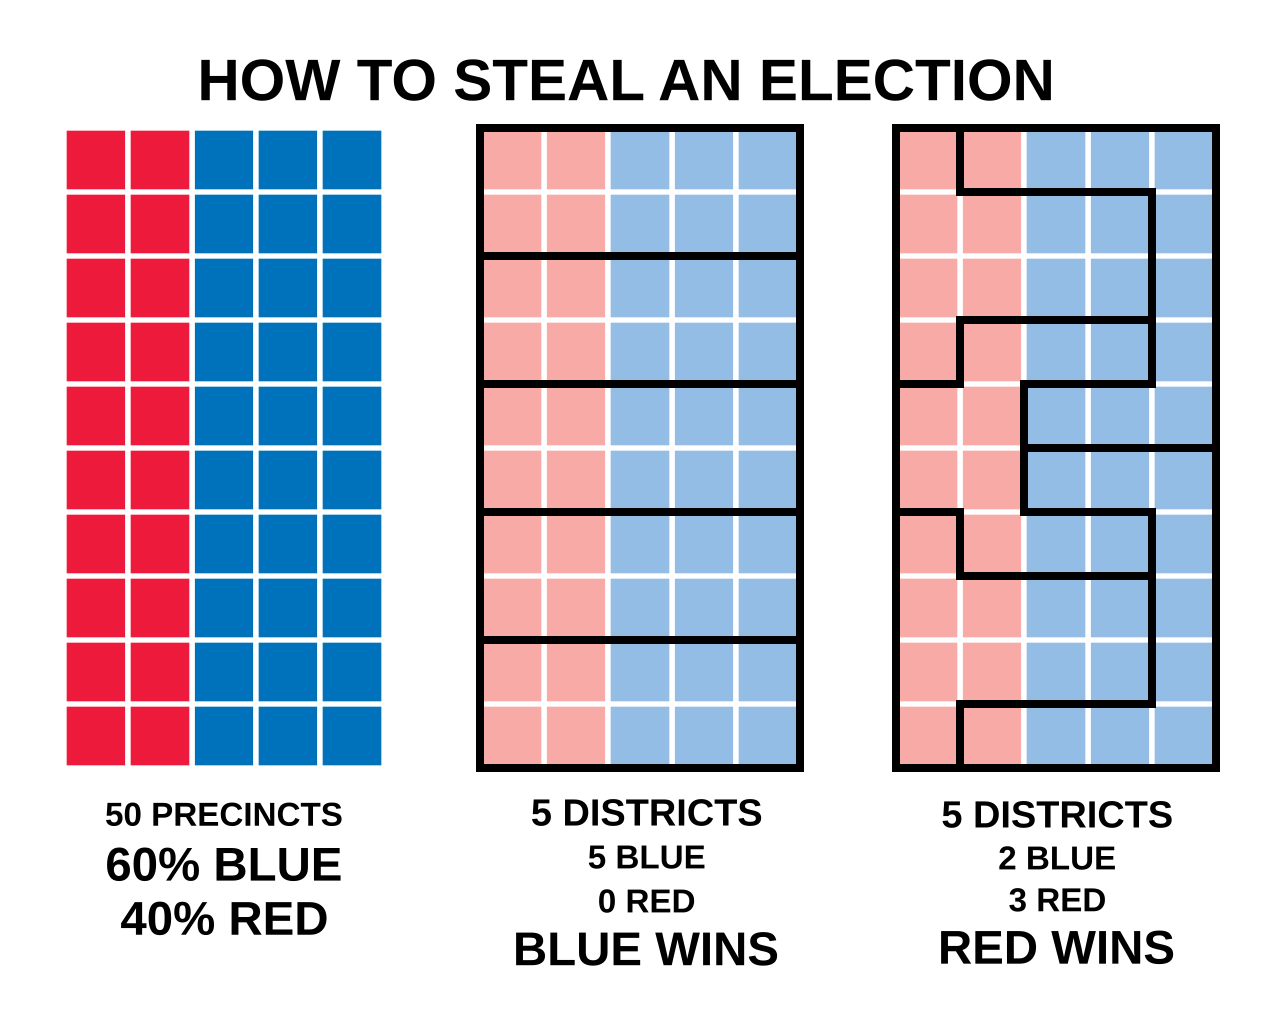
\includegraphics[width=\linewidth]{gerrymander.png}\\[0.1em]
      {\tiny\color{muted} Same voters, different maps. Diagram: Steve Nass, CC BY-SA 4.0\par}
    \end{column}
  \end{columns}
  \source{Source: Wikipedia, ``2025--2026 United States redistricting.''}
\end{frame}

\guess{How much was spent on\\political ads in 2026?}{\$11.6 billion}{The most expensive election ever. Elon Musk alone: at least \$474 million.}

% =====================================================================
\section{Ad Detective}

\begin{frame}{How to play}
  \begin{columns}[c]
    \begin{column}{0.58\textwidth}
      \begin{enumerate}\setlength{\itemsep}{1em}
        \item Watch the ad (30 seconds)
        \item \textbf{Vote:} positive or attack?
        \item \textbf{Vote:} which feeling?
        \item \textbf{Predict:} will it work?
        \item Write it down: answers come later!
      \end{enumerate}
    \end{column}
    \begin{column}{0.36\textwidth}
      \centering
      \renewcommand{\arraystretch}{1.6}
      \begin{tabular}{@{}c@{}}
        {\Large\bfseries\color{oldblue}Fear} \\
        {\Large\bfseries\color{oldred}Anger} \\
        {\Large\bfseries\color{dem}Laughter} \\
        {\Large\bfseries\color{navy}Trust} \\
      \end{tabular}
    \end{column}
  \end{columns}
\end{frame}

\adframe{1}{Maine Senate}{ad_collins.jpg}{hRLd5xuYOhs}{1\_collins.mp4}{
  \item \textbf{Made by:} Susan Collins (R)
  \item \textbf{Speaker:} Bill Green, a famous Maine TV reporter
  \item Mostly \alert{positive}, with a jab at Jackson: ``not about buying a cord of wood''
  \item Jackson's reply: it \emph{is} about wood --- heating costs}

\adframe{2}{Mississippi Senate}{ad_colom.jpg}{Nga2Q207-58}{2\_colom.mp4}{
  \item \textbf{Made by:} Scott Colom (D)
  \item \textbf{Target:} Sen.\ Cindy Hyde-Smith (R)
  \item Asked about high beef prices, she said: ``you have so many proteins''
  \item An attack using \alert{humor}}

\adframe{3}{Ohio Senate}{ad_brown.jpg}{PNQA4FuBqg0}{3\_brown.mp4}{
  \item \textbf{Made by:} Sherrod Brown (D)
  \item \textbf{Target:} Sen.\ Jon Husted (R)
  \item Says Husted took money from a friend of \alert{Jeffrey Epstein}
  \item Then voted to block the Epstein files}

\adframe{4}{North Carolina Senate}{ad_cooper.jpg}{cDHAxXWW4OM}{4\_cooper.mp4}{
  \item \textbf{Made by:} a Republican super PAC
  \item \textbf{Target:} Roy Cooper (D), former governor
  \item A grieving father blames Cooper's early prisoner releases
  \item \alert{Twist:} the father later said he was misled and would vote for Cooper (the PAC denies it)}

\adframe{5}{Texas Senate}{ad_paxton.jpg}{p3xRLG-_MOc}{5\_paxton.mp4}{
  \item \textbf{Made by:} Ken Paxton (R)
  \item \textbf{Target:} James Talarico (D), a former teacher who studies to be a pastor
  \item Real quotes from his sermons and podcasts
  \item Small print: parts made with \alert{AI}}

\adframe{6}{Ohio House, 7th District}{ad_miller.jpg}{pY9c2wPxI5o}{6\_miller.mp4}{
  \item \textbf{Made by:} a Democratic super PAC
  \item \textbf{Target:} Rep.\ Max Miller (R)
  \item Allegations of violence from news reports and his ex-wife (he denies them)
  \item No music, no jokes: pure \alert{fear}}

\adframe{7}{Bonus: Mayor of Los Angeles}{ad_pratt.jpg}{T4MHgjkdOKk}{7\_pratt.mp4}{
  \item \textbf{Made by:} Spencer Pratt, a reality-TV star
  \item \textbf{Target:} Mayor Karen Bass, shown as \alert{the Joker}
  \item Pratt is Batman; almost all of it is \alert{AI}
  \item 97 seconds long: three times a normal ad}

% =====================================================================
\section{The Results}

\begin{frame}{What Maine decided}
  \begin{columns}[c]
    \begin{column}{0.3\textwidth}
      \centering
      
\includegraphics[height=3.6cm]{jackson.jpg}\\[0.3em]
      {\bfseries\color{dem}Troy Jackson (D)}\\[0.1em]
      \uncover<2->{{\fontsize{24}{28}\selectfont\bfseries\color{dem}54\%}}
    \end{column}
    \begin{column}{0.3\textwidth}
      \centering
      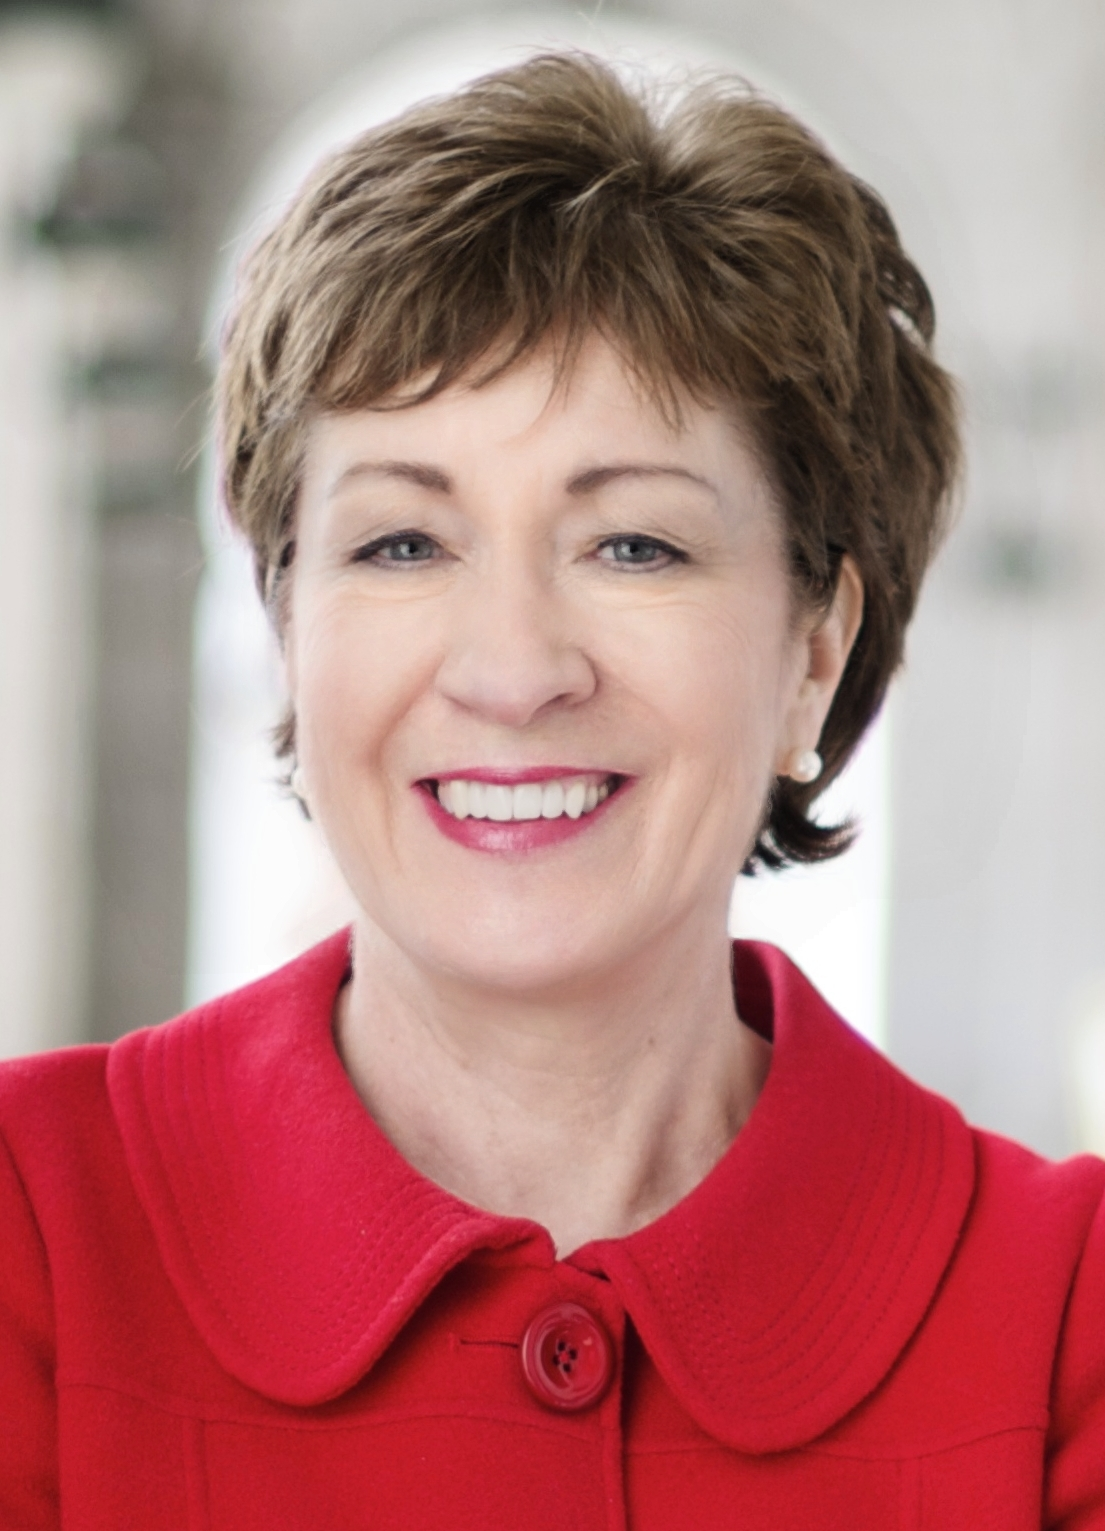
\includegraphics[height=3.6cm]{collins.jpg}\\[0.3em]
      {\bfseries\color{rep}Susan Collins (R)}\\[0.1em]
      \uncover<2->{{\fontsize{24}{28}\selectfont\bfseries\color{rep}46\%}}
    \end{column}
    \begin{column}{0.34\textwidth}
      \begin{itemize}\setlength{\itemsep}{0.8em}
        \item<2-> Collins out after \alert{30 years}
        \item<2-> A logger beat a famous senator
        \item<2-> How did \alert{our class} vote?
      \end{itemize}
    \end{column}
  \end{columns}
  \uncover<2->{\source{Source: NBC News, Nov.\ 4. Unofficial.}}
\end{frame}

\begin{frame}{Democrats win both chambers}
  \centering
  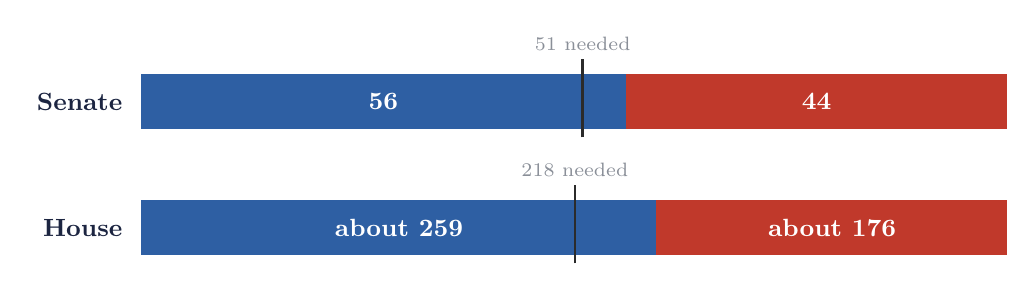
\begin{tikzpicture}[x=1.1cm, y=1cm,
      seg/.style={font=\small\bfseries, text=white},
      lab/.style={font=\scriptsize, text=muted}]
    % Senate: 100 seats mapped to 10 units
    \node[anchor=east, font=\small\bfseries, text=navy] at (-0.1,1.95) {Senate};
    \fill[dem] (0,1.6) rectangle (5.6,2.3);
    \fill[rep] (5.6,1.6) rectangle (10,2.3);
    \node[seg] at (2.8,1.95) {56};
    \node[seg] at (7.8,1.95) {44};
    \draw[ink, line width=0.9pt] (5.1,1.5) -- (5.1,2.5);
    \node[lab, anchor=south] at (5.1,2.48) {51 needed};
    % House: 435 seats mapped to 10 units
    \node[anchor=east, font=\small\bfseries, text=navy] at (-0.1,0.35) {House};
    \fill[dem] (0,0) rectangle (5.95,0.7);
    \fill[rep] (5.95,0) rectangle (10,0.7);
    \node[seg] at (2.98,0.35) {about 259};
    \node[seg] at (7.98,0.35) {about 176};
    \draw[ink, line width=0.9pt] (5.01,-0.1) -- (5.01,0.9);
    \node[lab, anchor=south] at (5.01,0.88) {218 needed};
  \end{tikzpicture}

  \vspace{1.2em}
  \begin{itemize}\setlength{\itemsep}{0.5em}
    \item Democrats flipped \alert{9 Senate seats}
    \item Most Democratic House seats since \alert{1993}
  \end{itemize}
  \source{Senate: AP, final calls Nov.\ 11 (Mississippi) and Nov.\ 17 (Alaska); 56 includes two independents. House: NBC News projection; a few races still counting as of Nov.\ 17.}
\end{frame}

\begin{frame}{Guess: who waited longest?}
  \relax{\small When did each state last elect a \textbf{\color{dem}Democratic} senator before 2026?\par}
  \vspace{0.6em}
  \centering
  \renewcommand{\arraystretch}{1.1}
  \begin{tabular}{@{}lc@{\hspace{1.6cm}}lc@{}}
    \toprule
    \textbf{State} & \textbf{Year} & \textbf{State} & \textbf{Year} \\
    \midrule
    North Carolina & \uncover<2->{2008} & Iowa           & \uncover<2->{2008} \\
    Texas          & \uncover<2->{1988} & Ohio           & \uncover<2->{2018} \\
    Maine          & \uncover<2->{1988} & Mississippi    & \uncover<2->{1982} \\
    South Carolina & \uncover<2->{1998} & Alaska         & \uncover<2->{2008} \\
    Kansas         & \uncover<2->{\alert{\textbf{1932}}} & & \\
    \bottomrule
  \end{tabular}

  \vspace{0.8em}
  \uncover<2->{Kansas: the first time in \alert{94 years}.}
  \source{The nine seats Democrats flipped in 2026. Source: U.S.\ Senate.}
\end{frame}

\begin{frame}{Did the ads work?}
  \centering
  \renewcommand{\arraystretch}{1.25}
  \begin{tabular}{@{}lllc@{}}
    \toprule
    \textbf{Ad} & \textbf{Made by} & \textbf{Result} & \textbf{Worked?} \\
    \midrule
    1 \; Maine         & Collins (R)      & \uncover<2->{Jackson 54, Collins 46}      & \uncover<2->{\color{oldred}\textbf{No}} \\
    2 \; Mississippi   & Colom (D)        & \uncover<3->{Colom by half a point}       & \uncover<3->{\color{dem}\textbf{Yes}} \\
    3 \; Ohio          & Brown (D)        & \uncover<4->{Brown 50, Husted 45}         & \uncover<4->{\color{dem}\textbf{Yes}} \\
    4 \; North Carolina & Republican PAC  & \uncover<5->{Cooper 59, Whatley 39}       & \uncover<5->{\color{oldred}\textbf{No}} \\
    5 \; Texas         & Paxton (R)       & \uncover<6->{Talarico 55, Paxton 43}      & \uncover<6->{\color{oldred}\textbf{No}} \\
    6 \; Ohio 7th      & Democratic PAC   & \uncover<7->{Miller lost, 45--55}          & \uncover<7->{\color{dem}\textbf{Yes}} \\
    7 \; Los Angeles   & Pratt            & \uncover<8->{3rd in June: out of the race} & \uncover<8->{\color{oldred}\textbf{No}} \\
    \bottomrule
  \end{tabular}

  \vspace{0.8em}
  \uncover<9->{Who in our class predicted the most correctly?}
  \source{Sources: AP; NBC News; Mississippi Today; CBS News; Los Angeles Times. Unofficial results, as of Nov.\ 17.}
\end{frame}

\begin{frame}{Does money buy elections?}
  \begin{itemize}\setlength{\itemsep}{1em}
    \item Texas: about \alert{\$300M} for Paxton, \$80M for Talarico
    \item Talarico still won \alert{by 12}
    \item Ads matter less than \alert{the mood}
    \item In 2026: an unpopular President, high prices
  \end{itemize}
  \vspace{0.6em}
  \begin{center}\textbf{\color{navy}Which ad would change \emph{your} vote?}\end{center}
  \source{Outside spending in the Texas Senate race: AdImpact via The Hill and Al Jazeera (late Oct.).}
\end{frame}

\begin{frame}{History repeated itself}
  \centering
  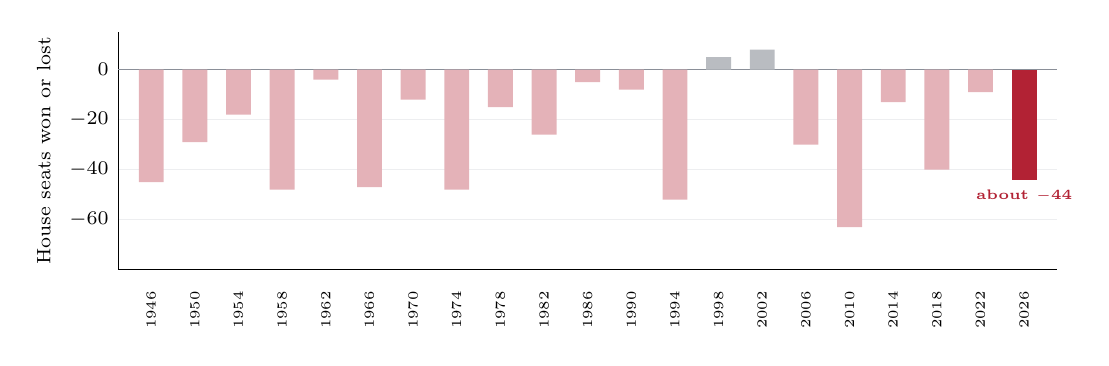
\begin{tikzpicture}
    \begin{axis}[
        ybar, width=13.5cm, height=4.6cm, bar width=9pt, clip=false,
        ymin=-80, ymax=15, xmin=1943, xmax=2029,
        axis x line*=bottom, axis y line*=left,
        xtick={1946,1950,...,2026}, x tick label style={font=\tiny, rotate=90, anchor=east, /pgf/number format/1000 sep={}},
        ytick={-60,-40,-20,0}, y tick label style={font=\scriptsize},
        ymajorgrids, grid style={navy!8},
        ylabel={\scriptsize House seats won or lost}, tick style={draw=none}]
      \draw[muted] (axis cs:1943,0) -- (axis cs:2029,0);
      \addplot[fill=oldred!35, draw=none, bar shift=0pt] coordinates {
        (1946,-45) (1950,-29) (1954,-18) (1958,-48) (1962,-4) (1966,-47) (1970,-12)
        (1974,-48) (1978,-15) (1982,-26) (1986,-5) (1990,-8) (1994,-52)
        (2006,-30) (2010,-63) (2014,-13) (2018,-40) (2022,-9)};
      \addplot[fill=muted!60, draw=none, bar shift=0pt] coordinates {(1998,5) (2002,8)};
      \addplot[fill=oldred, draw=none, bar shift=0pt] coordinates {(2026,-44)};
      \node[font=\tiny\bfseries, text=oldred, anchor=north] at (axis cs:2026,-44) {about $-$44};
    \end{axis}
  \end{tikzpicture}

  \vspace{0.3em}
  \begin{itemize}\setlength{\itemsep}{0.3em}\small
    \item The President's party lost, \alert{again}
    \item The map war backfired: Texas Republicans won only 1 of 5 new seats
    \item Top issues: \alert{the economy} (39\%), democracy (32\%)
  \end{itemize}
  \source{2026: NBC News projection (about 176 Republican seats) vs.\ 220 won in 2024. Texas: Texas Tribune. Issues: NBC News exit poll. Not final.}
\end{frame}

\begin{frame}{What happens next?}
  \begin{itemize}\setlength{\itemsep}{0.9em}
    \item New Congress starts \alert{January 2027}
    \item Trump stays President until \alert{2029}
    \item Democrats can investigate and block laws
    \item Trump can still \alert{veto} their bills
    \item Next big test: the \textbf{2028} presidential election
  \end{itemize}
\end{frame}

% =====================================================================
\section{Your Turn: Make an Ad}

\begin{frame}{Make a 30-second ad}
  \begin{columns}[c]
    \begin{column}{0.5\textwidth}
      \begin{enumerate}\setlength{\itemsep}{0.9em}
        \item In pairs, pick a candidate
        \item Positive or attack?
        \item Pick a feeling
        \item Write a slogan + script
        \item Perform it: class votes!
      \end{enumerate}
    \end{column}
    \begin{column}{0.46\textwidth}
      \centering
      {\small\bfseries\color{oldred}8 minutes}\\[0.8em]
      \begin{textquote}[fontupper=\itshape, halign=center]
        ``I'm \ldots, and I approve this message.''
      \end{textquote}
      {\footnotesize\color{muted} Every U.S.\ candidate ad must end like this\par}
    \end{column}
  \end{columns}
\end{frame}

\begin{frame}{Pick your candidate}
  \centering
  \card{\textbf{\color{oldred}A}}{A golden retriever}{for Mayor of Vienna}\hfill
  \card{\textbf{\color{oldred}B}}{A robot}{for class president}\hfill
  \card{\textbf{\color{oldred}C}}{A Viennese pigeon}{wants to ban tourists}\\[0.5em]
  \card{\textbf{\color{oldred}D}}{Your grandmother}{for Chancellor of Austria}\hspace{0.6cm}%
  \card{\textbf{\color{oldred}E}}{The Schnitzel Party}{free Schnitzel, no homework}
\end{frame}

\end{document}
